\documentclass{article}

\usepackage[backend=biber]{biblatex}
\addbibresource{BPGP.bib}

\usepackage{graphicx}
\graphicspath{ {./images/} }

\usepackage{listings}
\usepackage{hyperref}
\lstset{language=Java}          % javascript isn't supported, for now, use Java as replacement

\newcommand{\code}{\texttt}

\title{Source-Code Evolution: Closing the Gap Towards the Evolution of Entire Programs - Connect Four}
\author{Zvika Haramaty}
\date{\today}

\begin{document}

\maketitle


\section{GP}
Evolutionary algorithms are a family of search algorithms inspired by the process of (Darwinian) evolution in Nature. Common to all the different flavors of evolutionary algorithms is the notion of solving problems by evolving an initially random population of candidate solutions, through the application of operators inspired by natural genetics and natural selection, such that in time ``fitter'' (i.e., better) solutions emerge. The field, whose origins can be traced back to the 1950s and 1960s, has come into its own over the past few decades, proving successful in solving multitudinous problems from highly diverse domains including (to mention but a few): optimization, electronic circuit design, telecommunications, networks, finance, economics, image analysis, signal processing, music, and art. Evolutionary algorithms have also proven highly useful in combination with other machine-learning approaches.

A genetic algorithm is an iterative procedure that involves a population of individuals, each one
represented by (perhaps) a finite string of symbols, known as the \emph{genome}, encoding a possible solution in a given problem space. This space, referred to as the \emph{search space}, comprises all possible solutions to the problem at hand. The algorithm sets out with an initial population of individuals that is generated at random or heuristically. Every evolutionary step, known as a \emph{generation}, the individuals in the current population are \emph{decoded} and \emph{evaluated} according to some predefined quality criterion, referred to as the \emph{fitness}, or \emph{fitness function}. To form a new population, which will constitute the next generation, individuals are \emph{selected} according to their fitness, and then transformed via genetically inspired operators, of which the most well known are \emph{crossover} and \emph{mutation}. Crossover involves ``mixing'' two or more genomes to form novel offspring, and mutation randomly modifies symbols in the genomes. Continually iterating this procedure, and owing to the principle of selection of the fittest, the genetic algorithm may eventually find an acceptable solution, i.e., one with high fitness.

Genetic programming is essentially a GA wherein the population contains programs. The programs are often represented as recursive computational trees, constructed from \emph{functions} and \emph{terminals}. The main flow of a GP run is similar to that of a GA, and the primary difference lying in the genetic operators, performed on the individual trees in the evolving population.

GP is mostly used to define a more sophisticated genomic representation for the problem at hand,
rather than to evolve bona fide, full-fledged computer programs. This is (arguably) true not only where traditional
tree-based GP is concerned, but also for other forms of GP, e.g., linear GP, grammatical evolution, etc'.
In a comprehensive monograph surveying the field of genetic programming, Poli et al. noted that:

\begin{quotation}
While it is common to describe GP as evolving \emph{programs} [emphasis in original], GP is not typically used to evolve programs in the familiar Turing-complete languages humans normally use for software development. It is instead more common to evolve programs (or expressions or formulae) in a more constrained and often domain-specific language.
\end{quotation}

Recent surveys have underscored key problems in source-code evolution, and discussed the current
solutions along with their limitations.~\cite{Petke2018} surveyed the field of genetic improvement (GI) of software -
a special case of code evolution, where automated search, such as GP, is used for improving existing software.
\cite{Banzhaf2018}~surveyed code evolution in general. Here, we do not presume to provide a full survey of the field,
but merely to present the key issues that we will need to address. As we discuss below, we believe that we have found
the missing link that fills the gap for many of the current issues. According to~\cite{Banzhaf2018, Petke2018}
the problems and their current solutions are:

    {\Large TODO}

\section{BP}
    {\Large TODO}

    \subsection{Context BP}
    {\large TODO}

\section{Connect Four}
`Connect Four' was solved by Victor Allis at his Thesis~\cite{Allis}.
He describes the strategies that allow the first player to win, and the second player to at least get a draw.
\emph{(Moshe: There is also an inactive MIT course~(\cite{Gymrek2009}) that's based on his Thesis. Is it interesting
to mention here?)}
Later, the game was solved with brute force methods by~\cite{Tromp}.
In our work, we first set to write few strategies manually in the BP paradigm, in order to demonstrate its ability to
handle Connect Four.
Following that, we proceed with evolving the game strategies with GP technics.

\subsection{Manual Strategies}
\emph{Moshe: I've just recently found~\cite{Allis}, and haven't read much of it. I will update this section
later with insights from it.}

The initial strategy that we've demonstrated is ``take 5''.
\begin{figure}[h]
    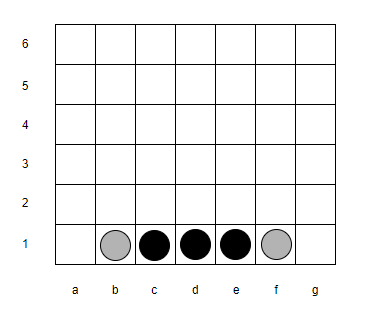
\includegraphics{five}
    \caption{``take 5'' strategy}
    \label{fig:take-5-strategy}
\end{figure}
As can be seen in figure~\ref{fig:take-5-strategy}, once a player has 3 adjacent pieces in a line \footnote{we use
\emph{line} to denote either \emph{row, column} or \emph{diagonal}}, and the 2 neighboring cells are empty, the
victory is inevitable. We capture this concept with the Contextual BThread demonstrated at
listing~\ref{lst:take-5-bt-lst}~/~
figure~\ref{fig:take-5-bt-fig}. All possible \emph{fives} are added as \emph{Context-BP entities}, and that BThread 
is instantiated for each of them, and killed once that entity deceases. Thus, for each possible \emph{five} in the 
board, a separate BThread is waiting trying to capture its center as long as it's still relevant, and then requests 
the winning last cell of the four in a line.

    {~\\ \large TODO - describe other strategy/ies}\\

This simple strategy easily wins a random player, but is hardly a much for any more sophisticated program. However, 
it serves well its purpose to demonstrate the feasibility of writing Connect-4 strategies with BP. 

\emph{Moshe: which way of displaying the code is better? using \emph{listing} or \emph{figure}?}

\lstinputlisting[caption=Five Strategy BThread, label={lst:take-5-bt-lst}, captionpos=b, firstline=172, lastline=181]{bl.js}

\begin{figure}[h]
    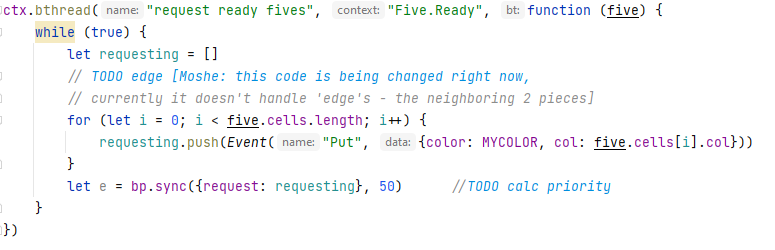
\includegraphics[width=\textwidth]{five_bt}
    \caption{``take 5'' Bthread - alternative}
    \label{fig:take-5-bt-fig}
\end{figure}


\subsection{Evolving Strategies}
In order to avoid to avoid bloat, typical to GP Koza-style trees, and in order to facilitate code generation, we've
used Grammatical Evolution (GE)~\cite{ONeill2001}. Since Context BP is implemented in Java, we've prefered to use
ECJ~\cite{Luke1998ECJSoftware}, the state-of-the-art Java EC library. The code is available at \url{https://github
.com/ZvikaZ/BPGP-First}

\subsubsection{Theoretical Grammar}

The grammar is of the format:
\begin{verbatim}
<start> ::= <bthread> | <bthread> <start>
<bthread> ::= BThread(<context> <priority>)
<context> ::= "Five.Ready" | "TODO"
<priority> ::= 50 | 60
\end{verbatim}

And the \code{BThread(context, priority)} function is defined as:

\begin{verbatim}
ctx.bthread("generated-code", context, function (five) {
    while (true) {
        let requesting = []
        for (let i = 0; i < five.cells.length; i++) {
            requesting.push(Event("Put", {color: MYCOLOR, col: five.cells[i].col}))
        }
        let e = bp.sync({request: requesting}, priority)
    }
})
\end{verbatim}

\emph{Moshe: This is of course a very primitive grammar, and will become more sophisticated later. I could have written
the previous grammar that I've used, before switching to Context BP - which looks better, but I figured it's pointless.}


\subsubsection{ECJ Grammar}
ECJ manual states that ``Each clause is a single GP node in Lisp s-expression form'', where each such GP node is
expected to be some function.
In other words, the design of ECJ encourages to implement the interpreter of the generated code directly in its
functions.
However, in our use case, we wanted to generate `dummy' text, that will be passed as-is to BPjs.

In order to achieve that, we've defined each GP node to return its relevant text (e.g., figure~\ref{fig:ecjc-bt}),
and also a \emph{cons} function (inspired by Lisp) that just concatenates together the texts (figure~\ref{fig:ecjc-cons}).

\begin{figure}[h]
    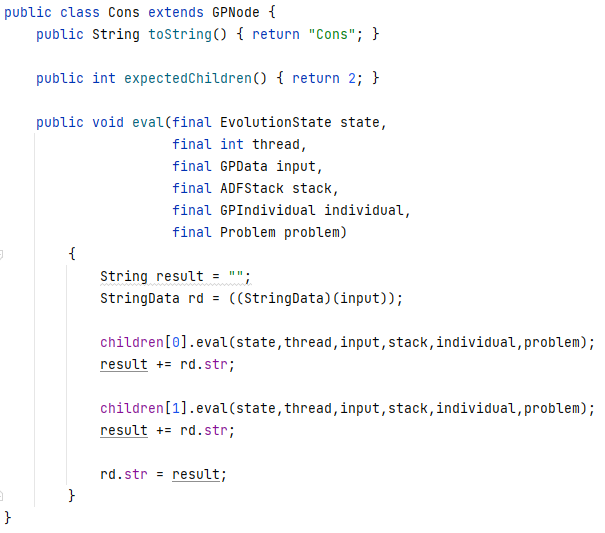
\includegraphics[width=\textwidth]{ecj-cons}
    \caption{`cons' implementation}
    \label{fig:ecjc-cons}
\end{figure}

\begin{figure}[h]
    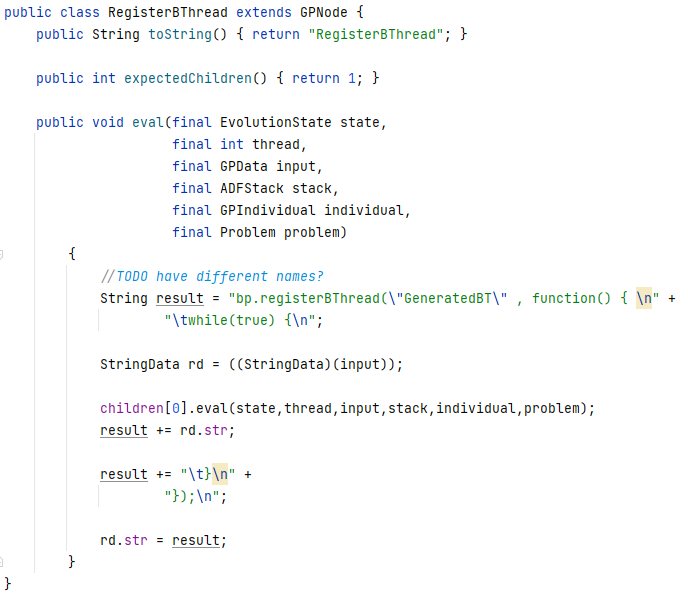
\includegraphics[width=\textwidth]{ecj-bt}
    \caption{`RegisterBthread' implementation}
    \label{fig:ecjc-bt}
\end{figure}


\subsubsection{Fitness}
We've few different fitness measures. The most basic one, which is more appropriate for the initial stages, is to play
40 games against random player,
giving 0 points for win, 1 point for draw and 2 points for loss (using Koza fitness - 0 is best, infinity is
worst).
For more advanced stages, it's helpful to play against other individuals in the population.
And in the final stages it's possible to play against an external program, using standard MiniMax with Alpha Beta
pruning~\cite{Scott}, with a small variation - in case of loss, the user gets \(2-\frac{num\_of\_plys}{6\cdot 7}\)
points, thus, the longer he has succeeded to postpone the loss, the better.

We combine the 3 different fitness measures differentially - in the beginning we're using only the first measure. And
as the fitness improves, we start to apply the other measures, with higher and higher weights.

\subsubsection{Recombination operators}
Currently we're using GA standard operators - 2 point crossover, and simple mutation.
We expect that in later phases we'll develop operators that are more suitable for our domain - with awareness
of BTs boundaries. Thus, the crossover will do exporation across BTs, and the mutation will do exploitation inside
the BT.


\printbibliography

\end{document}
